%Plot of n versus time for all implementations
%Effect of tuning parameters (how many copies?)
%Extrapolation of how long my data set would take with each?
%Actual result for my data set

We created a series of test cases of various sizes and ran our different implementations on Hopper. We checked the correctness of our implementations by comparing our results to results given by the R package \texttt{gstat} \cite{Pebesma} for the smaller test cases. We compiled the \texttt{C} code backing the R package on Hopper and ran the test cases in serial to get a baseline timing. [HOW THAT WENT***]

\begin{figure}[!h]
   \centering
   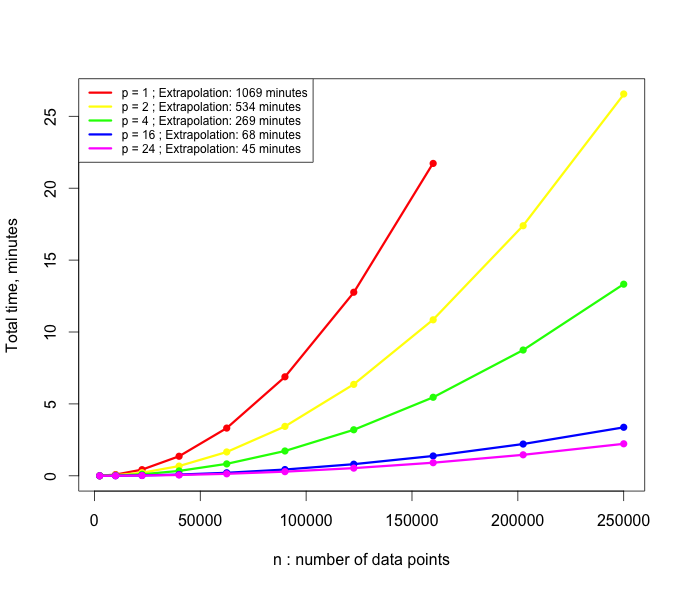
\includegraphics[width=0.75\textwidth]{./fig/comm_c1_timings.png} % requires the graphicx package
   \caption{For all 10 test cases, various numbers of processors in one node were timed and the curves represent the number of processors. A line was fit for the square root of time versus test case size and extrapolated to $n=8.69\times10^6$, the result listed in the legend). For this communication optimal implementation on one node, the large data set is still not reasonable.}
   \label{fig:comm_c1_timings}
\end{figure}

We executed 10 test cases for our communication-optimal and computational-optimal implementations for various numbers of processors. Figure~\ref{fig:comm_c1_timings} shows the timing results for our communication optimal implementation with the replication factor $c=1$. It depicts the distinctive $O(n^2)$ curve for the smaller number of processors $p$ (the horizontal axis is too small to show the shape of the curve for the larger $p$) and the expected reduction in time with increasing $p$. For each of these curves, we fit a line between total time and $n^2$ and then extrapolated the time required to run the large dataset of Figure~\ref{fig:herten} with $n=8.69\times10^6$. On the legend, the extrapolated time is written for each $p$ tested.  

Figure~\ref{fig:comm_allc_timings} compares $c=$ 1, 2, and 4. The effect of $c$ is not evident when looking at the total time. When breaking the total time down into time for reading the file, broadcasting the point data, shifting the point data, computing the squared differences, and reducing the bins (see Figure~\ref{fig:allc_breakdown}), it its evident that most of the total time is consumed by the computation stage. The effect of $c$ is more evident if only the shifting time is plotted (see Figure~\ref{fig:comm_allc_comm})

\begin{figure}[!h]
   \centering
   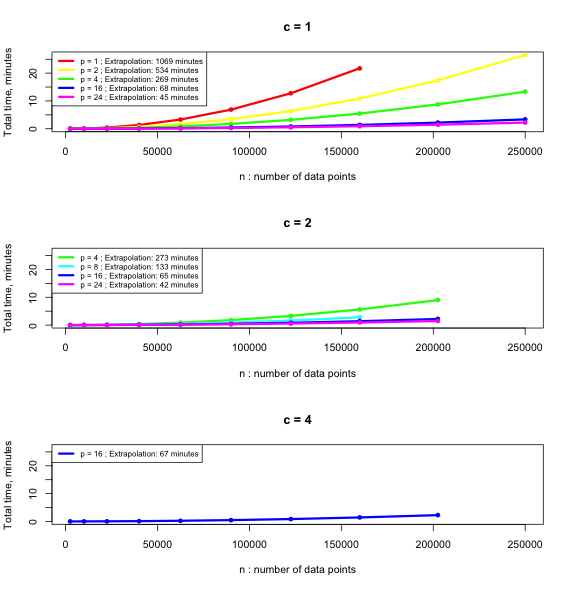
\includegraphics[width=\textwidth]{./fig/comm_allc_timings.png} % requires the graphicx package
   \caption{For all 10 test cases, various numbers of processors in one node were timed and the curves represent the number of processors. there is no detectable difference for the different values of $c$. }
   \label{fig:comm_allc_timings}
\end{figure}

\begin{figure}[!h]
   \centering
   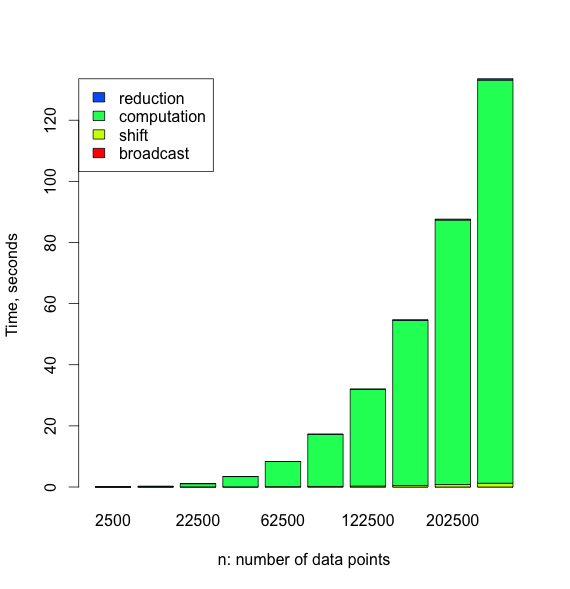
\includegraphics[width=0.75\textwidth]{./fig/comm_24_breakdown.png} % requires the graphicx package
   \caption{The breakdown of total time for executing our communication optimal code for 24 processors. The categories considered are shifting the data points, broadcasting the points, calculating the square differences, and reducing the bins. The collective communication calls of broadcast and reduce are effectively zero and computation dominates. }
   \label{fig:allc_breakdown}
\end{figure}

\begin{figure}[!h]
   \centering
   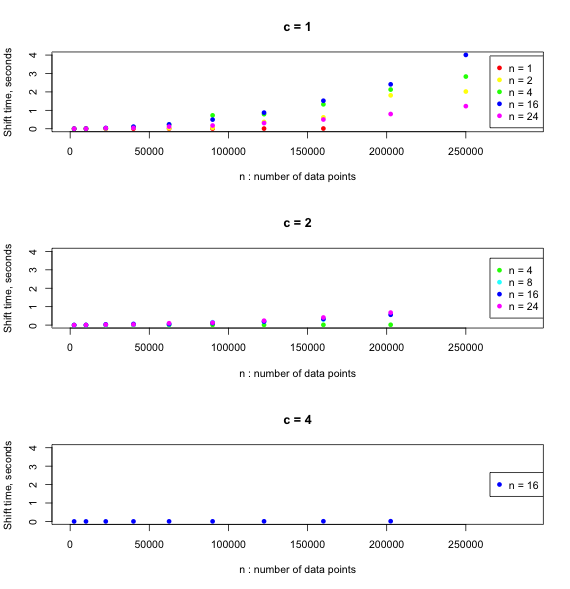
\includegraphics[width=\textwidth]{./fig/comm_allc_comm.png} % requires the graphicx package
   \caption{The time for shifting the data points around the processor teams in the communication optimal implementation is shown for different test case size and number of processors. With increasing $c$, the shifting time reduces, but there are less options for $p$ since $c^2$ needs to divide $p$ evenly. The effect of the replication factor $c$ is only seen for the shifting time and none of the other timing categories, however since computation out weighs communication the $c$ is not a tuning parameter we spent much time configuring.}
   \label{fig:comm_allc_comm}
\end{figure}

Due to computation consuming most of the total time, we next tried the computation optimal implementation. Figure~\ref{fig:comp_timings} shows the timing results for total time of our 10 test cases and for a range of processors. Again, the $O(n^2)$ curve is evident and we extrapolated the time required for our large data set. The total time for the computation optimal implementation is about half of that of the communication optimal implementation. Breaking down the total time for this computation optimal implementation (Figure~\ref{fig:comp_breakdown}), we can see that the file reading becomes the bottle neck  when increasing the number of processors. 

\begin{figure}[!h]
   \centering
   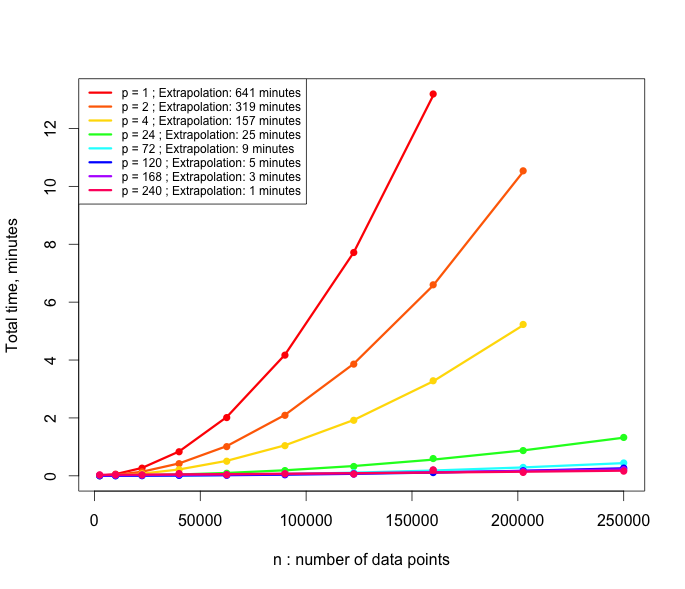
\includegraphics[width=0.75\textwidth]{./fig/timing.png} % requires the graphicx package
   \caption{For all 10 test cases, various numbers of processors in one node were timed and the curves represent the number of processors. A line was fit for the square root of time versus test case size and extrapolated to $n=8.69\times10^6$, the result listed in the legend). As to be expected, increasing the number of processors lowered the total time for each test case, and the effect is more pronounced with larger test cases. Although it doesn't appear that increasing the number of processors helps much after $p=72$, the effect would be more pronounced for cases larger than our test cases. }
   \label{fig:comp_timings}
\end{figure}

\begin{figure}[!h]
   \centering
   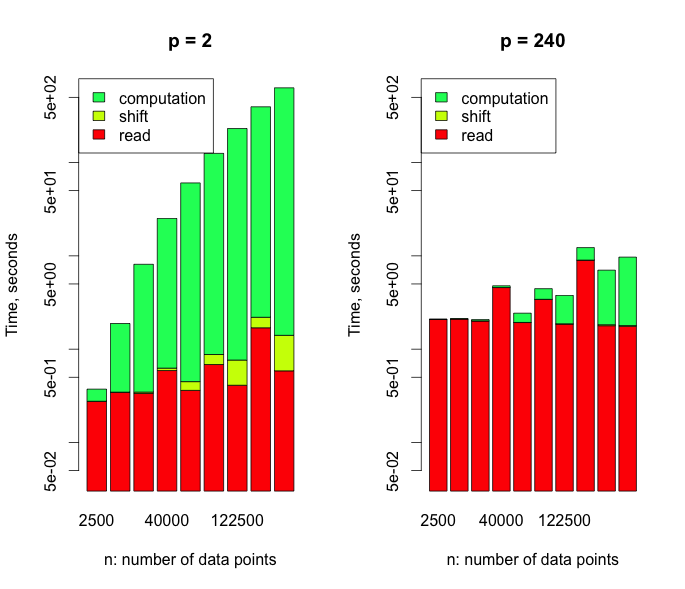
\includegraphics[width=0.75\textwidth]{./fig/comp_breakdown.png} % requires the graphicx package
   \caption{The log-scale breakdown of total time for executing our computation optimal code for 2 and 240 processors. The three categories considered are reading the file, shifting the data points, and calculating the square differences. The collective communication calls of broadcast and reduce are not included as they were effectively zero. For $p=2$ computation dominates, but for $p=240$, reading the file dominates.}
   \label{fig:comp_breakdown}
\end{figure}

Next, we looked at the scaling success (Figure~\ref{fig:scaling}). We divided the time $p=1$ by each larger $p$ and compared it to the $y=x$ line representing perfect scaling. It can be seen that for the larger test cases, there is near-perfect scaling for up to 144 processors. Although this is not the case for the smaller test cases, this is not really an issue because our program is designed for large data sets and small ones can be run in serial in reasonable time. 

\begin{figure}[!h]
   \centering
   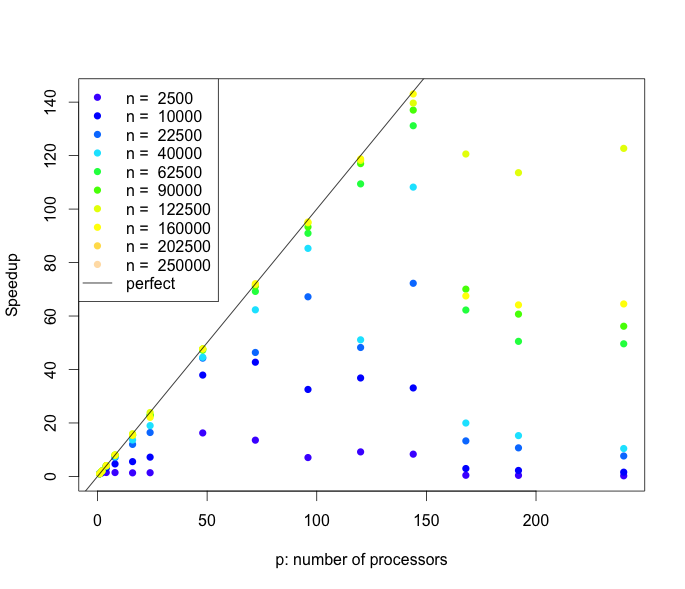
\includegraphics[width=0.75\textwidth]{./fig/speedup.png} % requires the graphicx package
   \caption{For all 10 test cases, various numbers of processors were timed and compared to the $p=1$ case for the respective test case size. larger test cases exhibit better scaling than smaller test cases, and using up to 144 processors showed near-perfect scaling.}
   \label{fig:scaling}
\end{figure}

Now that we are content with the performance of the computation optimal implementation, we increased $p$ and re-ran our test cases to determine the appropriate $p$ to run our large data set in a matter of seconds (instead of a day which is the quickest we could get with one node in our preliminary tests). Figure~\ref{fig:extrapolate} shows the extrapolated time for the large data set for  increasing number of nodes (each with 24 processors). ??????And which is a good amount???? 

\begin{figure}[!h]
   \centering
   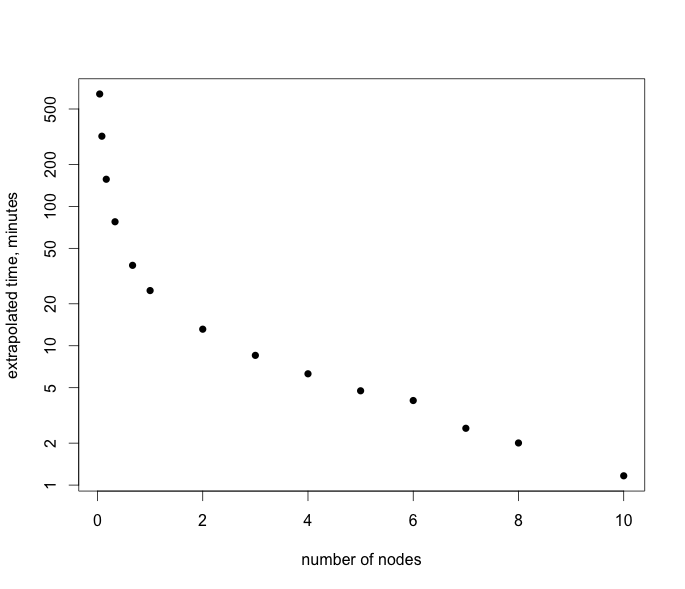
\includegraphics[width=0.75\textwidth]{./fig/extrapolate.png} % requires the graphicx package
   \caption{The log-scale extrapolated time to calculate the empirical variogram for $n=8.69\times10^6$ from a few processors in one node up to all 24 processors in 10 nodes. With the 10 nodes, it will only take one minute to calculate the variogram.}
   \label{fig:extrapolate}
\end{figure}
